\documentclass[11pt]{article}
\usepackage[margin=2.15cm]{geometry}
\usepackage{graphicx}
\usepackage{booktabs}
\usepackage{microtype}
\usepackage[numbers,sort&compress]{natbib}
\usepackage[hidelinks]{hyperref}
\usepackage{xcolor}
\usepackage{authblk}
\usepackage{lineno}
\usepackage{caption}
\definecolor{navy}{HTML}{173B57}
\definecolor{pending}{HTML}{9B2C2C}
\definecolor{pendingbg}{HTML}{FFF4F2}
\captionsetup{font=small,labelfont=bf}
\setlength{\parindent}{0pt}
\setlength{\parskip}{0.48em}
\emergencystretch=1em
\linenumbers

\newcommand{\resultpending}[2]{%
  \begin{center}
  \fcolorbox{pending}{pendingbg}{\parbox{0.91\linewidth}{%
    \textcolor{pending}{\textbf{#1}}\\[-0.1em]
    \small #2}}
  \end{center}}

\newcommand{\figurepending}[2]{%
  \begin{figure}[t]
  \centering
  \fcolorbox{pending}{pendingbg}{\parbox[c][4.2cm][c]{0.88\linewidth}{%
    \centering\textcolor{pending}{\textbf{#1}}\\[0.6em]
    \small #2}}
  \caption{\textbf{Reserved display item.} This panel remains blank until its preregistered evidence gate closes.}
  \label{#1}
  \end{figure}}

\title{\textbf{Replay-bound virtual chemistry benchmarks adaptive scientific agents}}
\author{\textbf{AUTHORS AND AFFILIATIONS PENDING}}
\date{Nature Computational Science Article working draft, 17 July 2026\\
\textcolor{pending}{Not for submission: formal method matrices and Bench evidence remain incomplete}}

\begin{document}
\maketitle

% ABSTRACT_START
\begin{abstract}
Autonomous scientific agents must choose experiments, act on partial observations and trade objective quality against safety, cost and information. Comparisons are difficult when algorithms receive different interfaces or when reported scores cannot be reconstructed from their actions. Here we introduce ChemWorld, a replay-bound virtual chemistry environment that exposes recipe optimizers, reinforcement-learning policies and tool-using language models to a shared typed contract. Fifteen task slices compose reaction, separation, crystallization, distillation, flow, electrochemical and equilibrium processes; six research tasks additionally support hidden world-family interventions. Every action is validated and committed transactionally, and a read-only evaluator recomputes endpoints, constraints, interaction capabilities and resource use from retained trajectories. Source-bound development matrices and reinforcement-learning preflights establish executability without accessing the sealed benchmark. Formal cross-method, generalization and transfer results are intentionally left open while their preregistered experiments are completed.
\end{abstract}
% ABSTRACT_END

Agents that automate scientific experiments face a sequential decision problem rather than a question-answering task. They must allocate a finite budget, decide when a measurement is worth its cost, act under operational constraints and use earlier outcomes to change later experiments. Physical self-driving laboratories demonstrate that such loops are feasible \citep{shields2021bo,szymanski2023alab,abolhasani2023sdl}, while tool-using language models can plan procedures and invoke chemistry software \citep{boiko2023coscientist,bran2024chemcrow}. Yet hardware, orchestration, measurement access and hidden human intervention often vary with the method being evaluated, making it difficult to attribute an apparent improvement to the agent itself.

Existing computational evaluations address complementary parts of this problem. Static chemistry benchmarks test knowledge and reasoning \citep{jablonka2024predictive,schneider2024chembench}; executable research benchmarks measure outcome and cost on data-analysis tasks \citep{chen2025scienceagentbench}; and virtual laboratories expose embodied operations \citep{beeler2024chemgymrl,li2025labutopia}. A remaining challenge is to compare heterogeneous adaptive agents under the same chemical state transitions while preserving enough evidence to reconstruct every score, constraint violation and resource claim.

ChemWorld addresses this challenge by separating five objects: an agent, a typed public interface, a hidden executable world, a read-only evaluator and a source-bound evidence layer. The public contract fixes what each interaction stratum can observe and do. Hidden world families vary executable laws without changing task semantics. The evaluator replays trajectories rather than trusting submitted summaries. Our study asks three questions: whether the contract remains operational across heterogeneous tasks and methods; whether learning and search methods can be frozen without consulting the sealed benchmark; and whether any final advantage survives private world shifts, exploit probes and independent reproduction. The first two questions can be addressed with current control and development evidence. Results for the third are left blank until the corresponding experiments close.

\section*{Results}

\subsection*{A typed contract makes heterogeneous agents auditable}

ChemWorld uses the Gymnasium interaction model \citep{towers2024gymnasium}, but its semantic action is a typed laboratory event rather than an unconstrained vector. A task publishes its allowed operations, instruments, parameter domains, budget and observable quantities. The validator checks the action against both this schema and the current public state before a domain service proposes a state patch. Constitution checks then cover non-negative material amounts, phase aggregation, vessel and equipment ownership, and mass and energy accounting. Only a valid patch is committed; failed operations remain visible in the trajectory.

The same interface supports three temporal strata. Recipe-search methods select a complete experiment and update between experiments. Operation-open-loop agents emit a sequence without intermediate feedback. Operation-closed-loop agents choose after every released observation. Capability is therefore reported alongside, rather than folded into, the endpoint. A system-level comparison can include different strata, but an algorithm-only claim requires matched information and interaction contracts.

Every trajectory binds the task, world allocation, public observations, actions, state-transition results and method resources. Evaluation reloads these records and recomputes task endpoints, risk, cost and validity. For online models, the evidence additionally includes provider identity, request parameters, tokens, retries, failures and monetary cost. Private chain-of-thought is neither required nor scored.

\begin{figure}[t]
  \centering
  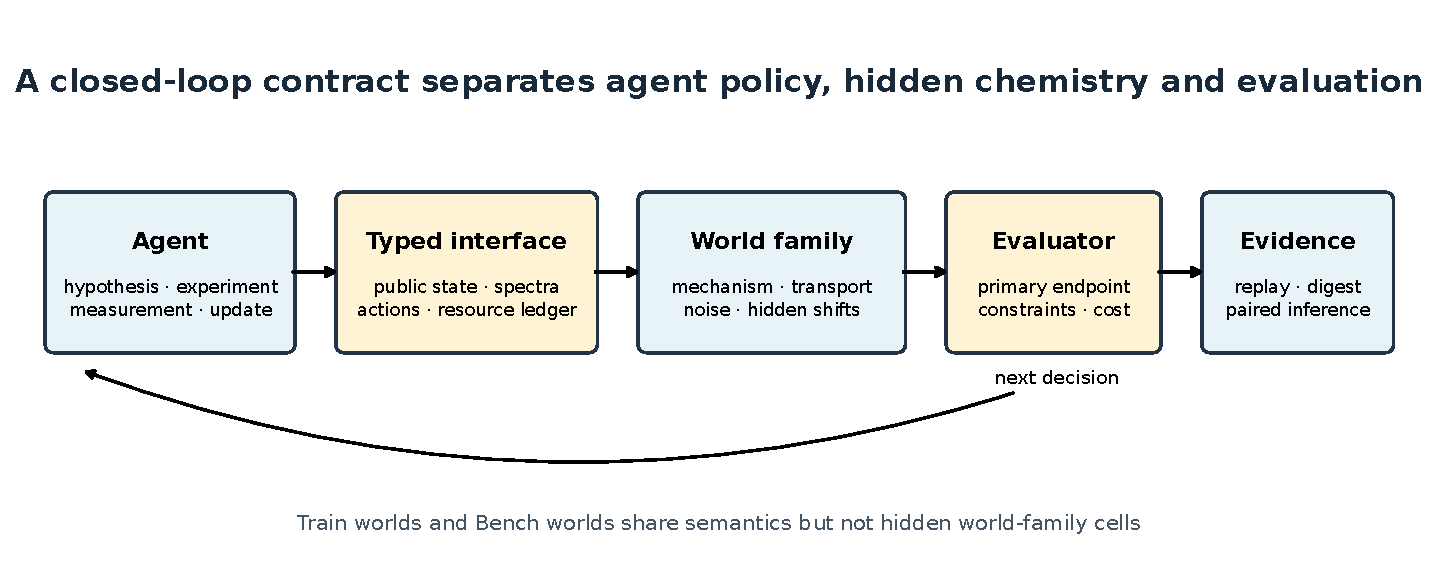
\includegraphics[width=\textwidth]{../figures/figure1_system.pdf}
  \caption{\textbf{Replay-bound architecture for virtual chemistry.} Heterogeneous agents act through one typed public contract. Hidden world families own executable mechanisms and observation models. A read-only evaluator reconstructs endpoints, constraints, interaction capability and resources from retained trajectories.}
  \label{fig:system}
\end{figure}

The environment registers fifteen task slices. Six research tasks cover liquid--liquid partition, reaction--crystallization, reaction--distillation, continuous-flow optimization, electrochemical conversion and equilibrium characterization. Four tasks form the preregistered comparison core; electrochemistry and equilibrium remain exploratory until their adaptive task-validity gates close. Registered functionality is consequently not treated as evidence that every task supports a defensible performance comparison.

\subsection*{Public affordances match executed runtime domains}

A heterogeneous benchmark can fail before any algorithm is compared if its published action domain disagrees with validation or execution. We therefore tested 223 boundary candidates across the six research tasks. The validator accepted 215, and all 215 committed through the runtime and remained inside their declared observation domains. The audit produced no schema--validator, validator--runtime or runtime--observation finding. This check included coupled constraints such as cooling rate, effective flow residence time, phase-dependent pressure and concentration, and the temperature and seed-population domains of cooling crystallization.

The control establishes that a valid public action is executable on the sampled boundaries; it is not a performance result. Physically legal programs that produce no useful material remain valid negative experiments rather than being relabelled as infrastructure failures. Conversely, an action outside a published constitutive domain fails before runtime instead of being silently clipped into a different experiment.

\subsection*{Development matrices freeze candidate method families}

Method development used only the public Train and Dev allocations. Three operation-level controls completed 288 preregistered cells, and eight classical recipe-search methods completed 768 cells; every cell contained forty complete experiments. Accounting, primary endpoints and decision audits were complete. Deterministic replay checks passed, and invalid actions from the operation-random control were retained rather than repaired. The classical matrix exercised random and Latin-hypercube design, local search, structured Gaussian-process and random-forest acquisition, and risk-constrained optimization.

These matrices were used to select representatives within preregistered method roles, not to report a winner. Bench feedback and reference-search feedback were unavailable. The retained development choices were Latin-hypercube design, greedy local search, structured GP--UCB, and structured safe GP--EI; all three operation-level controls remain because they represent distinct information contracts. Their final comparison is reserved for the sealed evaluation.

\subsection*{Reinforcement-learning preflights validate the training substrate}

The reinforcement-learning interface combines a public-affordance-masked categorical operation with operation-conditional parameters. The observation includes public process values, completed core-operation groups, the current operation mask and campaign progress. Training uses only public shaping signals: newly completed process requirements are rewarded once, invalid preconditions and premature closure are penalized, and the benchmark evaluator ignores the shaping return when recomputing the primary endpoint.

Source-bound preflights trained PPO and SAC on each of the four core tasks for 25,600 environment steps per task. Both algorithms completed 102,400 total steps and sixteen exact Dev replays. PPO showed a preregistered learning signal on four of four tasks and increased aggregate behaviour-complete experiments from 50 to 407. SAC showed a learning signal on three of four tasks and increased the same aggregate from 57 to 155. Both preflights had zero runtime-domain and observation-domain failures at step zero and after training.

These gates establish that the adapters can learn and execute under the current contract; they do not establish method readiness. PPO crystallization produced no trained behaviour-complete experiment in its preflight evaluation, despite improving the primary metric, and SAC distillation produced neither a trained behaviour-complete experiment nor a trained primary-metric observation. The multi-seed matrices must therefore satisfy the stricter candidate-eligibility rules rather than inheriting the aggregate preflight decision.

\resultpending{PENDING-RL-PPO}{Insert the four-task, five-seed PPO result only after the full matrix, checkpoint selection, resource ledger and deterministic replay report are complete.}

\resultpending{PENDING-RL-SAC}{Insert the matched SAC result only after its exact-source matrix and checkpoint index close. Do not pool the earlier quarantined SAC checkpoints.}

\figurepending{fig:PENDING-RL}{Planned content: task-level learning curves with preregistered checkpoints, eligible-seed counts and uncertainty across independent training seeds.}

\subsection*{Formal comparison remains sealed}

The method-freeze audit currently denies a Bench manifest because the reinforcement-learning matrices, final language-model scope and resource ceilings are incomplete. This fail-closed state prevents development observations from becoming post hoc benchmark selection. Reference portfolios will be generated independently only after the evaluated method identities, checkpoints, prompts and budgets are immutable.

\resultpending{PENDING-LLM}{Insert a language-model result only if the candidate and Dev protocol closes with frozen model access date, prompt, request parameters, failure accounting and cost. A single live diagnostic trajectory is not a comparison.}

\resultpending{PENDING-BENCH}{Reserved for the preregistered cross-method primary endpoints, simultaneous risk and cost decisions, and reference regret on the sealed Bench allocation.}

\resultpending{PENDING-GENERALIZATION}{Reserved for hidden mechanism-family shifts, exploit resistance and equal-budget adaptation analyses.}

\resultpending{PENDING-REPRODUCTION}{Reserved for independent clean-environment reproduction of the frozen result bundle.}

\figurepending{fig:PENDING-BENCH}{Planned content: task-by-method effect estimates and simultaneous objective--risk--cost decisions.}

\figurepending{fig:PENDING-GENERALIZATION}{Planned content: private-family generalization, exploit probes and independent reproduction.}

\section*{Discussion}

ChemWorld is designed to test adaptive scientific decision-making without treating a simulator score as chemical truth. Its main computational contribution is an executable separation between public interaction, hidden state transition, replayed evaluation and evidence release. This separation allows recipe optimizers, reinforcement-learning policies and tool-using language models to share task semantics while preserving differences in their interaction capability and resource use.

The current evidence supports three bounded conclusions. First, sampled public affordance boundaries align with validation, runtime and observation domains. Second, operation-level and classical development matrices can be completed with source-bound accounting without consulting Bench. Third, PPO and SAC can be trained and replayed under a common conditional action contract across the four core tasks. None of these controls establishes a formal method ranking. The missing multi-seed, live-model, sealed-Bench, hidden-family and reproduction results are deliberately visible in this draft rather than replaced by pilot estimates.

Several limitations will remain even if the pending experiments pass. The environment's constitutive families are bounded computational interventions, not a calibrated representation of all laboratory chemistry. Operational risk is a benchmark quantity rather than a laboratory safety guarantee. A ranking may depend on the published interaction stratum, experimental budget and method resource ceiling. Finally, transfer to physical systems requires an external bridge study; performance within ChemWorld cannot by itself establish real-world validity.

The benchmark is therefore intended as an auditable experimental instrument. A defensible final result must survive the same sequence as an experimental measurement: preregistration, controlled execution, retained raw records, independent recomputation and a claim boundary that does not expand after the outcome is known.

\section*{Online Methods}

\subsection*{Environment and transactional state transition}

A task declares its primary metric, allowed operations and instruments, episode mode, budgets, allocation and observation contract. State is held in typed species, phase, vessel, equipment, thermal, process and resource ledgers. Actions are canonicalized and checked against the public schema and stateful preconditions. A provider evaluates the requested physical or instrumental operation and returns a provisional patch. Constitution checks precede atomic commit; invalid patches are rolled back and retained as failed operations.

Unmeasured public quantities carry an explicit observation mask and are serialized as null rather than zero. Task scoring is separated from the online transition reward. Final endpoints are reconstructed from bound assay evidence and cannot be replaced by a model-supplied score.

\subsection*{Tasks, worlds and data separation}

The preregistered core comprises partition discovery, reaction to crystallization, reaction to distillation and continuous-flow reaction optimization, with product in the organic phase, crystal yield, distillate purity and flow conversion as primary metrics. Public Train worlds support implementation and fitting; public Dev worlds support frozen family and checkpoint selection. Bench worlds remain inaccessible until method freeze. Reference search uses an independent identity and random stream. Private world families perturb executable mechanisms or constitutive laws without altering the public task contract.

\subsection*{Agent interfaces}

Recipe-search agents select complete experiments and receive updates only between experiments. Operation-level agents act after each operation; the observation-blind, operation-random and rule controls differ in their access to measurement history. Classical methods use typed recipe coordinates with categorical material identities. The development candidates include random and space-filling designs, local search, structured surrogate acquisition and a risk-constrained GP.

PPO uses a native masked categorical distribution over valid public operations and a conditional diagonal Gaussian over the fields required by the selected operation. SAC retains a bounded continuous latent carrier decoded through the same public action contract; comparisons between the two are therefore system-level and disclose this decoder difference. Checkpoints bind algorithm, task, action, observation, reward and policy-distribution contracts by digest.

The language-model adapter requests one structured public decision per operation. Malformed output becomes a recorded model failure; the harness does not silently repair an action, finish an experiment or request a final assay. Provider usage is accounted across retries. Spectral masking removes spectral and chromatographic fields while retaining matched non-spectral context.

\subsection*{Reinforcement-learning reward and checkpoint selection}

Training reward preserves the raw environment reward and adds public process-progress terms. A core operation group earns 0.10 once, completing all groups earns 1.0, an invalid precondition incurs $-0.25$, premature closure incurs $-0.50$, and unsafe or high-cost steps incur additional penalties. Measurement itself has no bonus. The observation exposes the same public progress ledger so that progress-dependent reward is Markov.

For each RL algorithm, five model seeds are trained separately on each core task for 102,400 environment steps. Candidate checkpoints are retained at 25,600, 51,200 and 102,400 steps. A candidate is eligible only if all Dev episodes finish, all required process groups are completed, the primary metric is present, runtime and observation failures are zero, and all contract digests match. Eligible candidates are ranked by mean episode-best primary metric, then fewer training steps and lower model seed. The selected checkpoint must replay exactly twice.

\subsection*{Evaluation, resources and statistics}

Evaluation reports the task endpoint, risk and cost separately from training reward. It also retains invalid actions, runtime and observation failures, interaction diagnostics, environment steps, process CPU and GPU time, wall time, model calls, tokens and monetary cost where applicable. Resources are not collapsed into the endpoint score.

Formal comparisons are paired by task and world wherever the method contract permits. Task-specific smallest effects of scientific interest and simultaneous risk and cost rules are fixed before Bench access. Failed and incomplete cells remain in the denominator according to the protocol. Exact estimands, uncertainty intervals, multiplicity procedures and missingness rules will be inserted with PENDING-BENCH after the final protocol-bound report exists.

\subsection*{Replay, release and manuscript evidence}

Replay reloads the retained task, world, intervention and trajectory records, re-executes each operation and recomputes evaluation fields. Missing context, digest mismatch, non-finite output or score substitution fails closed. A release requires an immutable source identity, checkpoint or prompt digests, resource ledgers, source data, a clean-environment package and independent reproduction.

This manuscript is itself evidence-bound. The machine-readable ledger in \path{paper/ncs/evidence-ledger.json} records current control and development sources by SHA-256 and names every pending result artifact. A result placeholder is removed only after its required report passes its own gate. An AI coding assistant was used to help restructure draft prose, inspect repository evidence and implement manuscript checks. It is not an author; all scientific statements, analyses and final wording require verification and approval by the human authors before submission.

\section*{Data availability}

Versioned control, development and preflight reports used in the current draft are retained in the repository and bound in the manuscript evidence ledger. Formal Bench trajectories and source data will be deposited only after the sealed evaluation and disclosure review. \textcolor{pending}{PENDING: archival repository DOI and final data-release statement.}

\section*{Code availability}

The environment, agents, evaluators, replay tools and manuscript audits are maintained in the ChemWorld repository. Submission will cite an immutable release rather than a mutable branch. Credentials, private salts and sealed evaluation parameters will not be included in public artifacts. \textcolor{pending}{PENDING: release tag, archive DOI and clean-install reproduction identifier.}

\section*{Acknowledgements}

\textcolor{pending}{PENDING: author-approved acknowledgements and funding statement.}

\section*{Author contributions}

\textcolor{pending}{PENDING: author-approved CRediT statement.}

\section*{Competing interests}

\textcolor{pending}{PENDING: declarations from all authors.}

\bibliographystyle{unsrtnat}
\bibliography{../references}

\end{document}
